%%%%%%%%%%%%%%%%%%%%%%%%%%%%%%%%%%%%%%%%%%%%%%%%%%%%%%%%%%%%%%%
%
% Welcome to Overleaf --- just edit your LaTeX on the left,
% and we'll compile it for you on the right. If you open the
% 'Share' menu, you can invite other users to edit at the same
% time. See www.overleaf.com/learn for more info. Enjoy!
%
%%%%%%%%%%%%%%%%%%%%%%%%%%%%%%%%%%%%%%%%%%%%%%%%%%%%%%%%%%%%%%%

% ===============================================
% MATH 790: Real Analysis           Spring 2022
% hw_template.tex
% ===============================================

% -------------------------------------------------------------------------
% The preamble that follows can be ignored. Go on
% down to the section that says "START HERE" 
% -------------------------------------------------------------------------

\documentclass{article}

\usepackage[margin=1in]{geometry} 
\usepackage{amsmath,amsthm,amssymb,hyperref}
\usepackage[hangul]{kotex}
\usepackage[shortlabels]{enumitem}
\usepackage{booktabs, multicol, multirow} % Allows the use of \toprule, \midrule and \bottomrule in tables
\usepackage{graphicx, subfig} 

\newcommand{\R}{\mathbf{R}}  
\newcommand{\Z}{\mathbf{Z}}
\newcommand{\N}{\mathbf{N}}
\newcommand{\Q}{\mathbf{Q}}

\renewcommand{\labelenumii}{\arabic{enumi}.\arabic{enumii}}
\renewcommand{\labelenumiii}{\arabic{enumi}.\arabic{enumii}.\arabic{enumiii}}
\renewcommand{\labelenumiv}{\arabic{enumi}.\arabic{enumii}.\arabic{enumiii}.\arabic{enumiv}}

\newenvironment{theorem}[2][Theorem]{\begin{trivlist}
\item[\hskip \labelsep {\bfseries #1}\hskip \labelsep {\bfseries #2.}]}{\end{trivlist}}
\newenvironment{lemma}[2][Lemma]{\begin{trivlist}
\item[\hskip \labelsep {\bfseries #1}\hskip \labelsep {\bfseries #2.}]}{\end{trivlist}}
\newenvironment{exercise}[2][Exercise]{\begin{trivlist}
\item[\hskip \labelsep {\bfseries #1}\hskip \labelsep {\bfseries #2.}]}{\end{trivlist}}
\newenvironment{problem}[2][Problem]{\begin{trivlist}
\item[\hskip \labelsep {\bfseries #1}\hskip \labelsep {\bfseries #2.}]}{\end{trivlist}}
\newenvironment{question}[2][Question]{\begin{trivlist}
\item[\hskip \labelsep {\bfseries #1}\hskip \labelsep {\bfseries #2.}]}{\end{trivlist}}
\newenvironment{corollary}[2][Corollary]{\begin{trivlist}
\item[\hskip \labelsep {\bfseries #1}\hskip \labelsep {\bfseries #2.}]}{\end{trivlist}}

\newenvironment{solution}{\begin{proof}[Solution]}{\end{proof}}

\begin{document}

% ------------------------------------------ %
%                 START HERE                  %
% ------------------------------------------ %

\title{기말고사} % Replace with appropriate title
\author{경제정의와 불평등} % Replace "Author's Name" with your name
\date{\today}

\maketitle

% -----------------------------------------------------
% The following two environments (theorem, proof) are
% where you will enter the statement and proof of your
% first problem for this assignment.
%
% In the theorem environment, you can replace the word
% "theorem" in the \begin and \end commands with
% "exercise", "problem", "lemma", etc., depending on
% what you are submitting. 
% -----------------------------------------------------
\begin{enumerate}[{\bf 문제 \arabic*.}]
    \item 경제적 불평등이 경제성장에 부정적 영향을 줄 수 있는 가능성에 대하여 설명하시오.
    \item 그림 \ref{fig}\는 어떤 가구소득의 누적분포를 가구주 부모의 교육수준별로 나누어 나타낸 그림이다.
        \begin{figure}
            \centering
            \subfloat[\centering ㄱ국]{{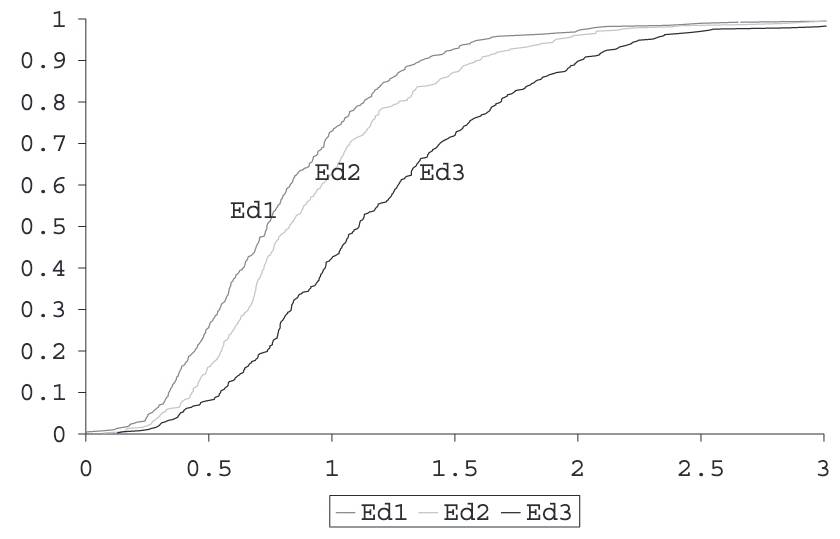
\includegraphics[width=0.45\textwidth]{pic/eopusa.png} }}%
            \qquad
            \subfloat[\centering ㄴ국]{{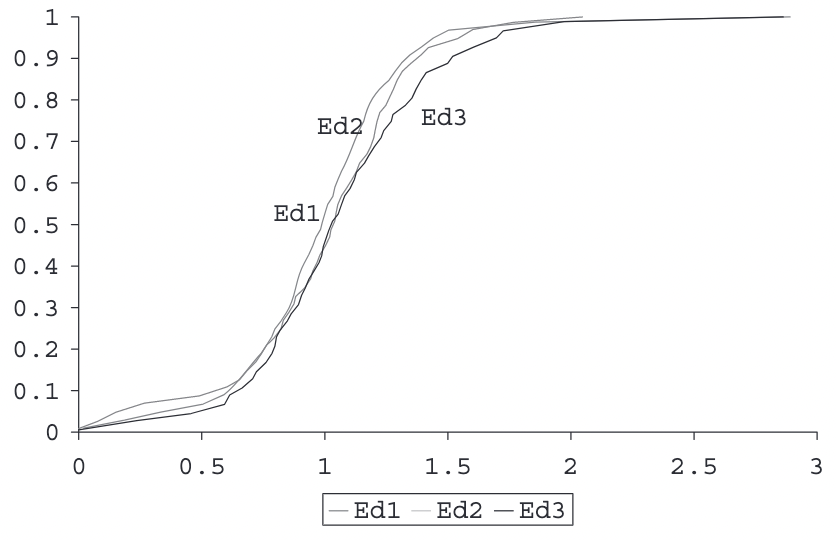
\includegraphics[width=0.45\textwidth]{pic/eopswe.png} }}%
            \caption{국가별 기회불평등 비교}%
            \label{fig}
        \end{figure}
        \begin{enumerate}
            \item 기회불평등 개념에서 말하는 환경에 대하여 정의하고 그 예시를 제시하시오.
            \item 각각의 국가에서 기회불평등의 존재여부를 답하고 설명하시오. 
            \item 본인이 Ed3이라는 환경에 속할때 어떤 국가에서 사는 것이 좋을 지에 대하여 설명하시오.
        \end{enumerate}
    \item 분배적 정의와 관련된 다음의 철학 문제에 대하여 답하시오.(각각 최대 5줄)
        \begin{enumerate}
        \item 하이에크(F. Hayek)로 대표되는 우파적 자유주의자의 분배적 정의에 대하여 설명하시오.
        \item 롤즈(J. Rawls)로 대표되는 파적 자유주의자의 분배적 정의에 대하여 설명하시오.
        \item 두 사상에서 제시하는 분배적 정의와 이를 실현하기 위한 사회제도 간의 관계에 대하여 각각 설명하시오.
        \end{enumerate}
    \item 최근 국내에서 300톤의 물을 대중공연에 사용한 것을 두고 논란이다.(각각 최대 5줄)
        \begin{enumerate}
            \item 우파적 자유주의의 입장에서 이러한 분배가 정의로운지 여부에 대하여 논하시오.
            \item 좌파적 자유주의의 입장에서 이러한 분배가 정의로운지 여부에 대하여 논하시오.
            \item 분배적 정의의 관점에서 본인의 생각을 논하시오.
        \end{enumerate}
    \item 4차산업혁명이 가져올 소득분배의 변화에 대하여 설명하시오.(최대 10줄)
\end{enumerate}

\end{document}